% Very simple template for lab reports. Most common packages are already included.
\documentclass[a4paper, 11pt]{article}
\usepackage[utf8]{inputenc} % Change according your file encoding
\usepackage{graphicx}
\usepackage{url}
\usepackage{listings}
\usepackage[listings]{tcolorbox}
\usepackage{xcolor}
\usepackage{xcolor}
\usepackage{float} 
\usepackage{placeins} 

% Define a custom boxed listing environment
\newtcblisting{mylisting}{
  colback=gray!5!white, colframe=black!75!white,
  listing only,
  left=2mm, right=2mm, top=1mm, bottom=1mm,
  boxrule=0.5pt, arc=2mm
}

%opening
\title{Report 4 - Groupy: Group Membership Service}
\author{Lorenzo Deflorian}
\date{\today{}}

\begin{document}

\maketitle

\section{Introduction}
The main goal of the assignment was to implement a group membership service providing atomic multicasting in view syncrony, while also tolerating crash failures.

\section{Main problems and solutions}
\subsection{Dancing together}
Group communication in our implementation relies on a leader-based protocol. The leader is responsible for maintaining a consistent view of the group membership and multicasting messages to all members. When a peer wants to join, it sends a request to the leader, who then updates the group view and shares it with everyone. The view consists of two parts: the list of all \textbf{process identifiers in the group}, and the list of \textbf{process identifiers at the application layer}.

Peers that are not the leader act as slaves. They forward join requests and multicast instructions to the leader, and also relay messages from the leader to the application layer. This setup ensures that all group members have the same view and that messages are delivered reliably, even if some processes crash.

Using our first implementation gms1, we can see that the group communication works as expected and all the peers change the colors in sync. However if the leader crashes the whole system stops working.

\subsection{Handling failures to keep on dancing}
To address the issue of leader crashes, we use monitors to detect failures. Each peer monitors the leader, and if it detects that the leader has crashed, it initiates a leader election process to select a new leader from the remaining members. The new leader then takes over the responsibilities of maintaining the group view and multicasting messages.

With this system in place we can see that if the leader crashes, one of the slaves takes over and the system continues to function without interruption. The group members continue to change colors in sync, demonstrating that the group communication is resilient to leader failures.

The implementation of gms2 shows the presented improvements and the system can handle leader crashes effectively.

\subsection{Actually we cannot dance}

While our gms2 implementation handles leader crashes effectively, it fails to guarantee true view synchrony when failures occur during message broadcasting. To demonstrate this limitation, we introduced random crashes in the broadcast function (gms2p5), where the leader might crash after sending a message to only some slaves.

This creates a critical problem: when the leader crashes mid-broadcast, some group members receive the message while others don't, leading to inconsistent states. Even after a new leader is elected, the group remains permanently out of sync because there's no mechanism to detect or recover from partial message delivery. This violates the reliability property of view synchrony, which requires that if any correct node delivers a message, all correct nodes must deliver it.

\begin{figure}[H]
  \centering
  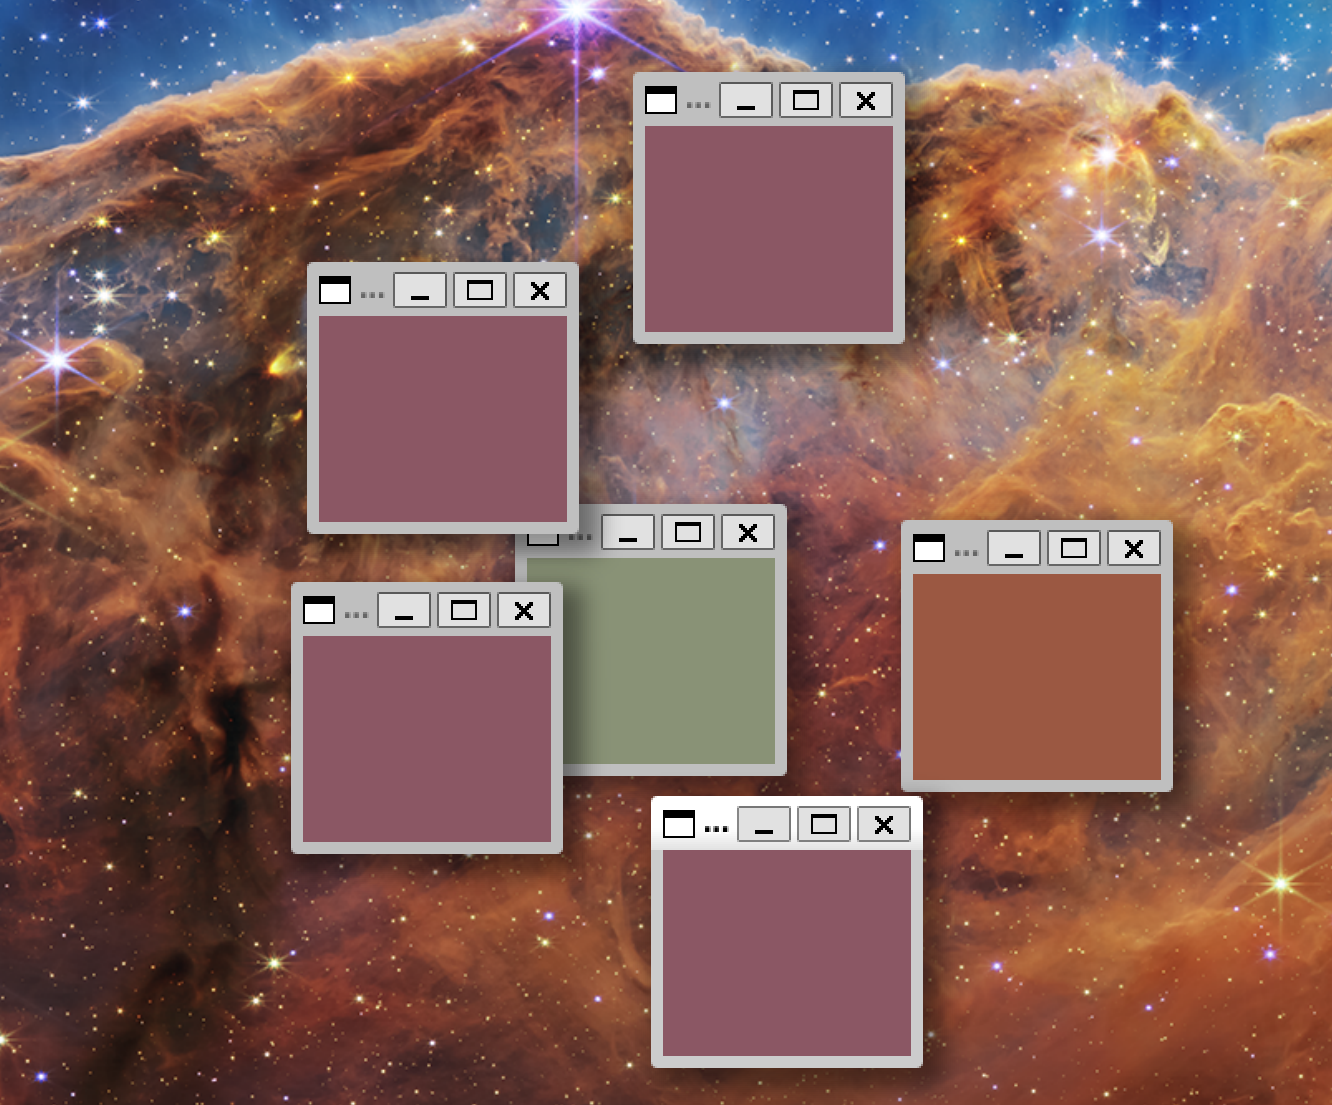
\includegraphics[width=0.7\textwidth]{imgs/out_of_sync.png}
  \caption{Peers out of sync after crash mid-broadcast.}
  \label{fig:out_of_sync}
\end{figure}

\subsection{Being more reliable dancers}
Starting from some assumptions we can implement a more robust multicasting protocol to address the issue where the leader crashes during message broadcasting.

Assuming that messages are reliably delivered and thus if the leader sends a message to S1 and then to S2 and S2 receives it, then S1 must have received it too, hence if one of the peers has received the message it means that for sure the first peer in the list has received it too.

When the leader crashes during the multicast procedure we can assume that some of the slaves might have not received the message. But keeping track of the last received message, when the new leader is elected it can send the last message again to all slaves, hence syncronizing also the ones that did not receive it the first time.

To avoid receiving the same message twice, hence shifting forward the state of the application we can introduce sequence numbers in our messages, so that if a peer receives a message with a sequence number lower or equal to the last one received it can just ignore it.

The implementation of gms3 shows the presented improvements and the system can handle leader crashes effectively while also guaranteeing view synchrony.

\section{Conclusions}

\end{document}